\chapter{Basics of response modeling}

\section{Amorphous track models}
ATMs (in a slightly confusing manner also referred to as 'track structure
models') started from the works of Robert Katz in the late 1950s. He and his
team worked on finding magnetic monopoles in nuclear emulsions exposed to
high-altitute cosmic radiation (TODO Ref.). Soon, \ldots

ATMs rely on two major assumptions:

\begin{itemize}
\item{They disregard the stochastic energy deposition pattern by secondary
electrons around the track of heavy charged particles (protons or
ions, HCPs). Instead, the averaged dose $d$ as a function of
distance $r$ from the trajectory is considered. $d(r)$ is mostly referred as the
'radial dose distribution' although the term 'distribution' is not fully correct
(Fig. \ref{fig:TST}).}
\item{The second important assumption is that -- since photons deposit their
energy eventually by electrons as well -- local radiation effects are supposed
to be the same for photons and HCPs.}
\end{itemize}
Thus, the response to irradiation with particles of type $T$ and energy $E$ can
be predicted from the homogenous bulk photon dose response $S_X(D)$ of the
detector system \cite{Katz_et_al_1972, Waligorski_and_Katz_1980}.

\begin{figure*}
	\centering
		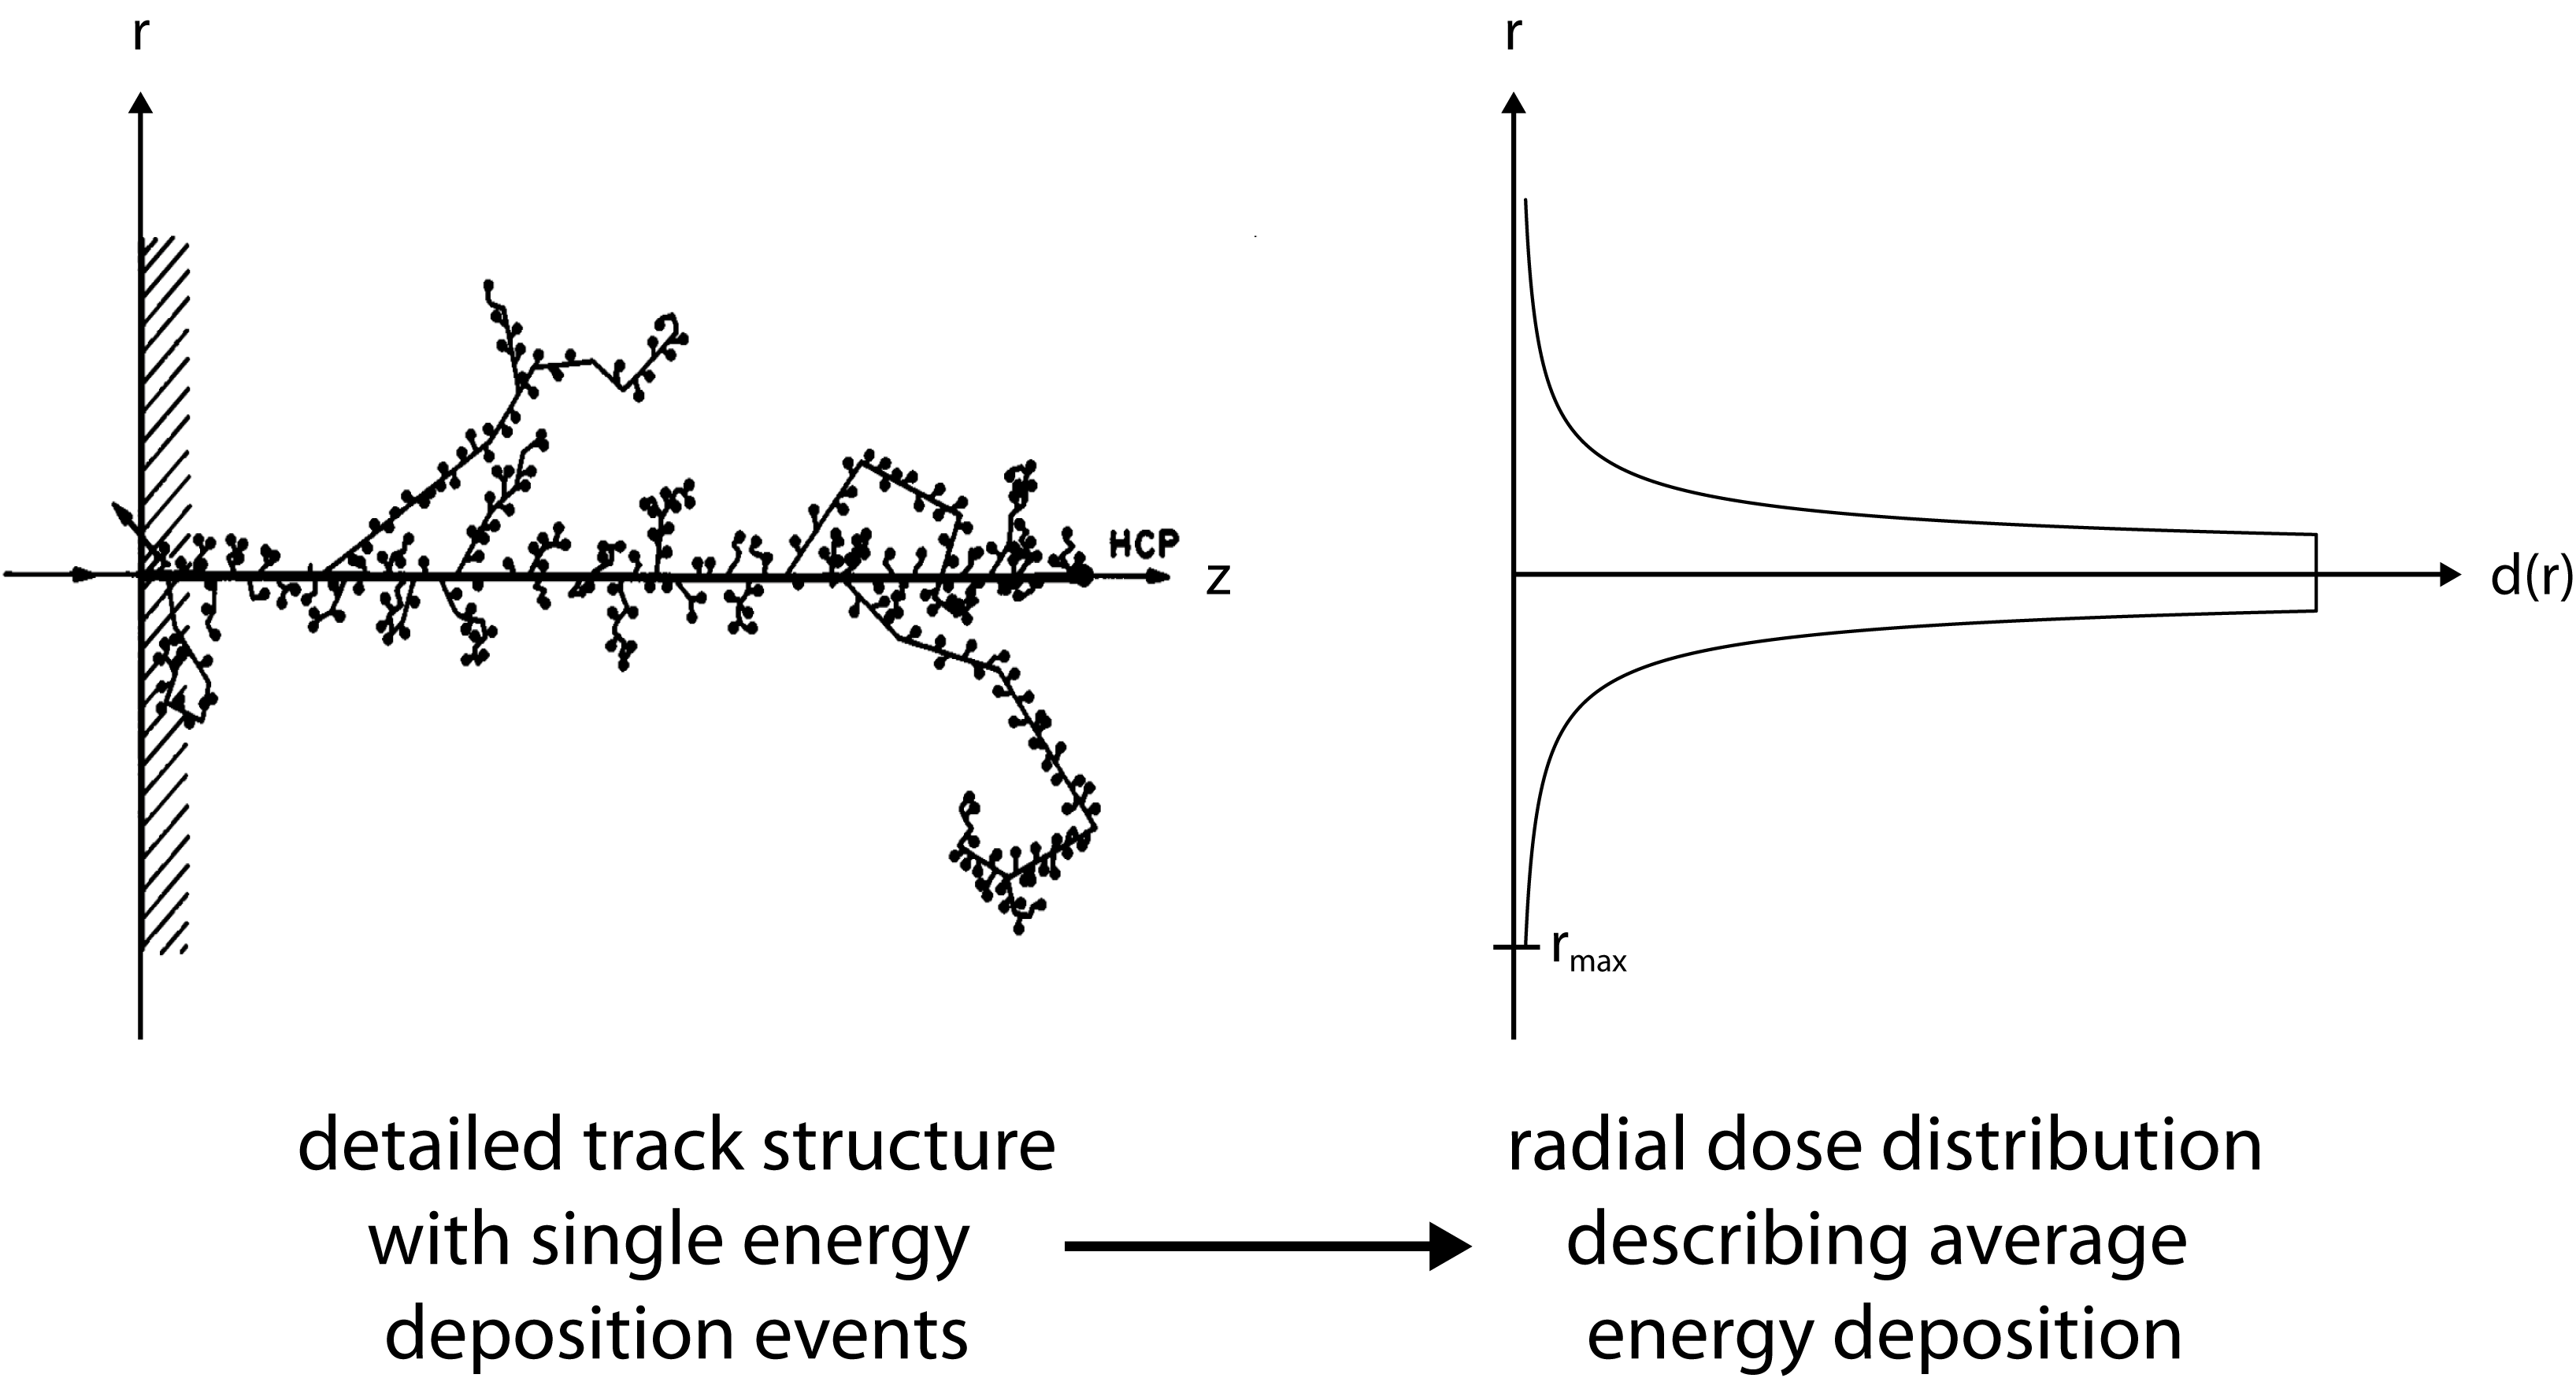
\includegraphics[bb=0 0 3271 1750,width=1.0\textwidth]{pictures/TrackStructureDetailAndRDD.png}
	\caption{Amorphization of the detailed track structure.}
	\label{fig:TST}
\end{figure*}


\section{Microdosimetric models}
Rossi, Kellerer - Theory of dual radiation action.
Olko

\section{Hybrid models}
Combining dual radiation approach (dose pattern in the sensitive target, the
nucleus e.g.) with ATM (to derive the pattern). Mathematically, a problem to
combine gamma and local dose. Solution discriminates approaches:
\begin{itemize}
  \item{LEM Arc segments, but problem. So: Scholz, 1992\ldots{} 1997 Single
  track, input parameter \cite{Geiss_et_al_1997, Bassler_et_al_2008}.}
  \item{GSM, iGSM/dGSM}
  \item{SPIFF}
\end{itemize}

\section{Averaging}
It is a bit confusing to see where averaging steps are taken in ATMs. A full
scenario would cover -- in three dimenions -- the stoachistic nature of energy
deposition in the functional subunits, placement of tracks, number and type of tracks. To
simplify this ATMs take the following steps:
\begin{itemize}
  \item Consider only the 2D situation perpendicular to the beam direction with
  a slice thickness according to the track segment regime.
  \item \textbf{First averaging} -- The stoachistic nature of the track is
  replaced by the radial dose distribution, i.e. the average of a large
  number of tracks, a representative track.
  \item \textbf{Second averaging} -- The stoachistic placement of the tracks is
  replaced by the integration over all possible impact parameters, weighted by
  their likelihood.
  \item \textbf{Third averaging} -- The random nature of multiple tracks
  affecting a functional unit (following a Poisson distribution) has to be
  tackled. In mixed fields, the tracks can also be of different subsets (30%
  protons, 70% Carbon etc.). 
\end{itemize}
Sometimes (LEM0), these steps are used to factorize the overall effect
($E=E_1\cdot E_2\cdot E_3$). But this assumes that no interaction (e.g.
$E_2\ast E_3$) is present. In the case of overlapping tracks
this is clearly not true!


\section*{Document status}
\begin{tabular}{l l}
2011.01.21&Created by S. Greilich
\end{tabular} 